\chapter{PANOC algorithm}
	This section is based on \cite{LorenzoStella2017} and \cite{AjaySathya2017}, the big difference is that this text is focused implementation. And so the formula's often look slightly different. The FBE part is based on \cite{Themelis}.
	\subsection{Introduction}
		The PANOC algorithm is an accelerated version of the proximal gradient descent. The direction  $x-\bar{x}$ calculated with the proximal gradient descent  is combined with a second direction, who will hopefully accelerate the convergence of the algorithm.
		
		\begin{equation}
		x_{k+1} = x_k - (1-\tau_k)\cdot (x-\bar{x}) + \tau_k d_k
		\end{equation}
		
		The new term $\tau_kd_k$ should accelerate the convergence if $\tau_k\neq0$. The step $d_k$ is calculated using a quasi-newton algorithm. As a quasi-newton algorithm uses curvature information of the cost function, it uses information not available to a gradient descent based method. 
		
		Furthermore it has a super linear convergence rate. Which is much faster then the sub-linear convergence of a typical gradient descent algorithm when it gets close to the solution. On top of that, the quasi-newton method will not require extra function evaluations. Which are the major contributors to the costs of the algorithm.
		
	\subsection{Quasi newton method}
		\subsubsection{Problem definition}
			The iteration of equation~\ref{eq:prox grad method} can indirectly be used to solve the optimization problem.  By using the residue defined in equation~\ref{eq:residue prox grad method} a fixed point can be found. 
			
			\begin{equation}
			R_{\gamma}(x)= \frac{1}{\gamma}\left[ x - \prox_g( x - \nabla f(x)\gamma) \right]
			\label{eq:residue prox grad method}
			\end{equation}
			
			The solution of equation~\ref{eq:residue prox grad method} can be found trough the Newton iteration of equation~\ref{eq:newton iteration residual}. Where $H_k$ satisfies the inverse secant condition of equation~\ref{eq:newton iteration residual inverse secant}. As the implementation is aimed at embedded software a good option to solve this would be LBFGS.
			
			\begin{equation}
			x^{k+1} = x^k -H_kR_{\gamma}(x^k)
			\label{eq:newton iteration residual}
			\end{equation}
			\begin{equation}
			x^{k+1} - x^k = H_{K+1} \Big( R_{\gamma}(x^{k+1})- R_{\gamma}(x^k) \Big)
			\label{eq:newton iteration residual inverse secant}
			\end{equation}
		\subsubsection{LBFGS}
			The variation of LBFGS used to solve equation~\ref{eq:LBFGS problem} is algorithm~\ref{alg:LBFGS}, the first iteration is not displayed.(the direction is equal to the gradient) And the current\ buffersize will increase every iteration from 1 to the limit specified by the controller designer.
			\begin{equation}
				R(x) = \frac{1}{\gamma}\left[ x - \prox_g( x - \nabla f(x)\gamma) \right] = 0
				\label{eq:LBFGS problem}
			\end{equation}
			\begin{algorithm}
				\caption{LBFGS}
				\label{alg:LBFGS}
				\begin{algorithmic}[1]
					\Procedure {LBFGS}{$x^k$,M=current\_buffersize}
					\State $q = R(x^k)$
					\For{i=M:1}
						\State $\alpha(i)=\rho(i) \cdot s(:,i)^Tq$
						\State $q = q - \alpha(i) \cdot y(:,i)$
					\EndFor
					\State $H_k^0 = y(:,M) \cdot s(:,M)^T \cdot  \frac{1}{y(:,M)^T \cdot y(:,M)}$
					\State $H^0_k \cdot R(x^k)$
					\For{i=1:M}
						\State $\beta(i) = \rho(i) \cdot y(:,i)^T \cdot z$
						\State $z = z + s(:,i)[\alpha(i)-\beta(i)]$
					\EndFor
					\For{i=1:M-1}
						\State $s(:,i+1)=s(:,i)$
						\State $y(:,i+1)=y(:,i)$
					\EndFor
					\State $$\begin{cases}
								s(:,1) = x_{k+1} - x_k \\
								y(:,1) = \nabla f(x_{k+1}) - \nabla f(x_k)\\
								\rho_k(1) = \frac{1}{y(:,1)^T \cdot s(:,1)} \\ 
							\end{cases}
							$$
					\State \Return direction=$-z=-H_k \cdot R(x^k)$
					\EndProcedure
				\end{algorithmic}
			\end{algorithm}
		
	\subsection{Forward backward envelop}	
		Newton iterations only converge quickly when they are close to the solution. In order to get better global behavior a proper global strategy is required. The optimization problem is changed from $\varphi(x) = f(x) + g(x)$ to equation~\ref{eq:FBE definition using Moreau envelope}. This problem is smoother while it still has the same optimal solution.(proof see \cite{LorenzoStella2017} and \cite{Themelis}) The same $\gamma$ as with the proximal gradient should be used, notice how the FBE contains the line-search condition use in the proximal gradient. (more on the FBE in \cite{Themelis})
		
		The Moreau envelope is de define as \ref{eq:Moreau envelope}, this smooths the function, and has a close relationship with the proximal operator as illustrated earlier. Using simple algebra equation~\ref{eq:FBE definition using Moreau envelope} can be transformed into equation~\ref{eq:FBE definition using quadratic approximation}.(proof in Appendix) The solution $y$ of the infimum defined in equation~\ref{eq:FBE definition using quadratic approximation} is $\bar{x}$. Considering the close relationship between the Moreau envelope and the proximal operator (see more in \cite{Themelis}) this is to be expected.
		
		An alternative way to look at it is nicely illustrated in \cite{AjaySathya2017}, where the problem can be seen as minimizing a quadratic approximation in point x.  Remember that $L = \frac{1}{\gamma}$, and L is the Lipschitz constant of the gradient.
		
		\begin{equation}
			g^{\gamma} = \underset{y}{\inf} \big \{f(y)+\frac{1}{2 \cdot \gamma}||x-y||^2 \big \}
			\label{eq:Moreau envelope}
		\end{equation}
		
		\begin{equation}
		\varphi_{\gamma} = f(x) - \frac{\gamma}{2}||\nabla f(x)||^2 + g^{\gamma} \big(x-\gamma \nabla f(x) \big)
		\label{eq:FBE definition using Moreau envelope}
		\end{equation}
		
		\begin{equation}
		\varphi_{\gamma} =   f(x) + \underset{y}{\inf} \Big\{ \nabla f(x)^T(y-x) + g(y) + \frac{1}{2 \gamma} ||x-y||^2  \Big\}
		\label{eq:FBE definition using quadratic approximation}
		\end{equation}
		
		\begin{proof}
			The solution to the infimum of equation~\ref{eq:FBE definition using quadratic approximation} is y=$\bar{x}= \prox_g(x-\gamma \nabla f(x))$
			\begin{align*}
			\prox_g(\bar{x}) 
			&=\prox_g(x- \gamma \nabla f(x)) \\
			&= \underset{y}{\argmin} \Big \{ g(y) 
			+ \frac{1}{2 \gamma}||(y-x) + \gamma \nabla f(x)||^2 \Big \} \\
			&= \underset{y}{\argmin} \Big \{ g(y) 
			+ \frac{1}{2 \gamma} \big[||y-x||^2 + 2 \gamma \nabla f(x)^T(y-x) + ||\nabla f(x)||^2\gamma^2 \big] \Big \} \\
			&= \underset{y}{\argmin} \Big \{ g(y) 
			+ \frac{1}{2 \gamma} \big[||y-x||^2 + 2 \gamma \nabla f(x)^T(y-x)  \big] \Big \}\\
			&= \underset{y}{\argmin} \Big \{   \nabla f(x)^T(y-x)  + g(y) 
			+ \frac{1}{2 \gamma} ||y-x||^2  \Big  \}
			\end{align*}
			\label{prf:prox is solution to FBE inf}
		\end{proof}
		
		Equation~\ref{eq:practical implementation of FBE} is the practical implementation of the FBE. The parameter gamma is the line-search parameter used in the proximal gradient descent. The first 3 terms are the same as with the line-search on $\gamma$, the last term $g(\bar{x})$ is new and makes sure the solution complies with the constraint.
		
%		\cite{AjaySathya2017} has an excellent example to illustrate this.(figure~\ref{fig:FBE illustration}).
%		
		\begin{equation}
			\begin{aligned}	
				& \varphi(\gamma,x)= 
				&& f(x) - \nabla f(x)^T(x-\bar{x}) + \frac{1}{2 \gamma}||x-\bar{x}||^2  + g(\bar{x})
				\\
				& with 
				&&\bar{x} = \prox_g( x - \gamma\nabla f(x)) 
			\end{aligned} 
			\label{eq:practical implementation of FBE}
		\end{equation}
		
%		\begin{figure}[H]
%			\centering
%			\label{fig:FBE illustration}
%			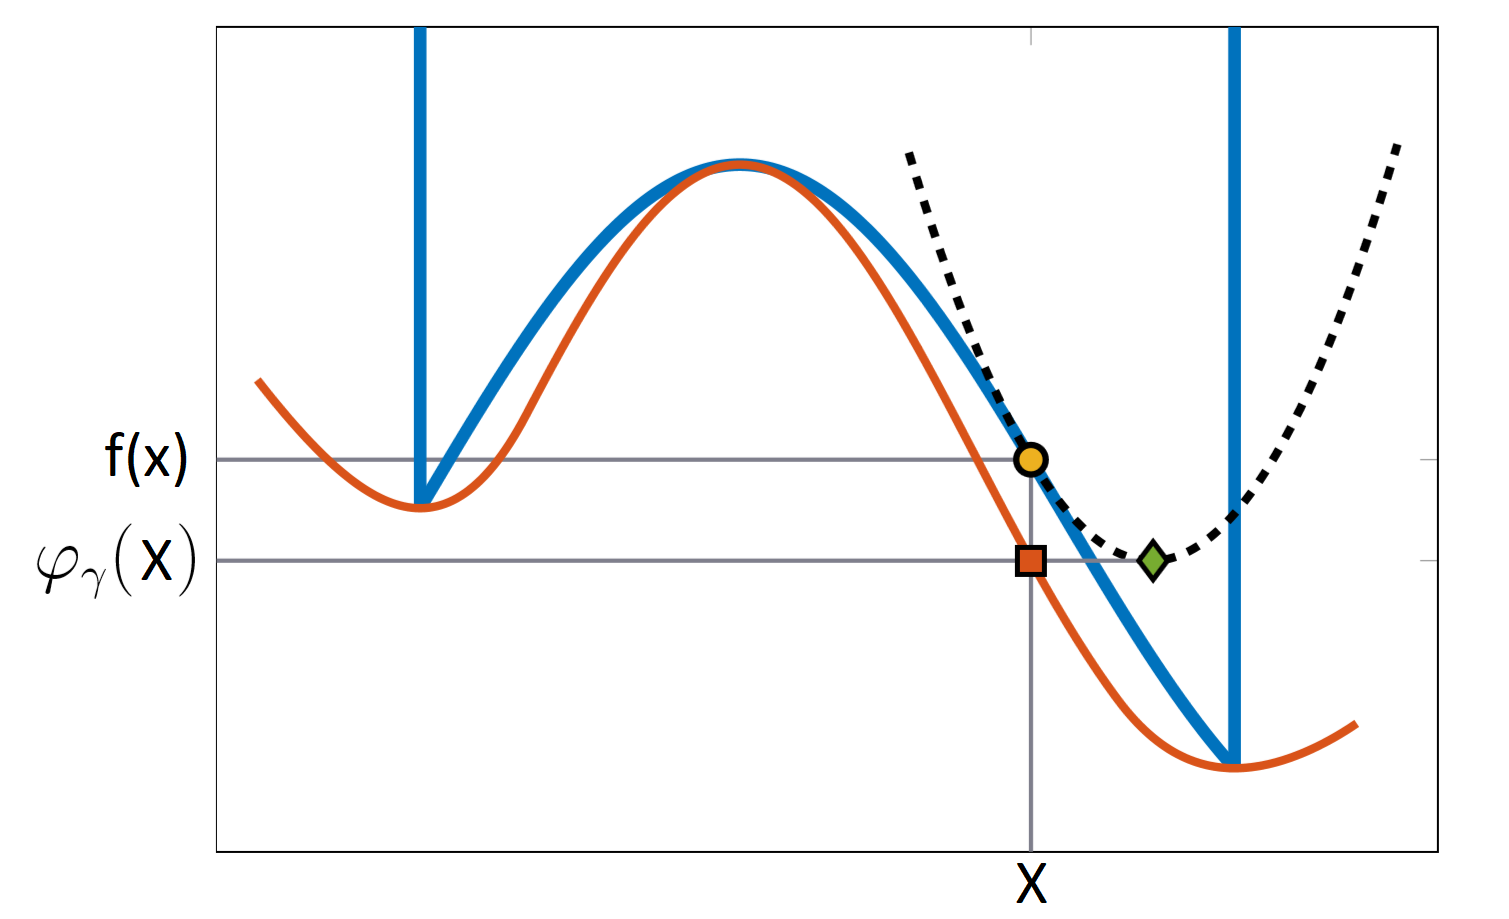
\includegraphics[width=0.6\textwidth]{FBE}
%			\caption{FBE example copied over from \cite{AjaySathya2017}, red is?? blue is ?? TODO expain this figure}
%		\end{figure}
	
	\subsection{Line-search with FBE}
	In \cite{LorenzoStella2017} the line-search condition is specified as equation ~\ref{eq:line-search with FBE}. The line-search parameter determines $x^{k+1}$ by choosing the convex combination of the step from the proximal gradient and the LBGFS as defined in equation~\ref{eq:linea-search tau definition}. It is also specifies in \cite{LorenzoStella2017} that $\sigma \in (0, \gamma \frac{1-\gamma\cdot L}{2})$. As stated before it is assumed that $L=\frac{1-\beta}{\gamma}$, some simple algebra will lead to the condition $\sigma \in (0,\frac{\beta \gamma}{2})$.
	
	 Equation~\ref{eq:practical line-search with FBE} is the practical implementation of equation~\ref{eq:line-search with FBE}. A new constant $\alpha \in (0,1)$ is introduced, an possible value for $\alpha$ would be 0.5 ($\alpha=0.5$ is the choice used by the Matlab implementation of PANOC in ForBes).
	
	\begin{equation}
		x^{k+1} = u_k - (1-\tau_k)\cdot (x-\bar{x}) + \tau \cdot dir_{LBFGS}
		\label{eq:linea-search tau definition}
	\end{equation}
	
	\begin{eqnarray}
		\label{eq:line-search with FBE}
		\varphi_{\gamma}(x^{k+1})\leq\varphi_{\gamma}(x^{k}) - \sigma ||\frac{x-\bar{x}}{\gamma}||^2 \\
		=
		\varphi_{\gamma}(x^{k}) - \frac{\sigma}{\gamma^2} ||x-\bar{x}||^2
	\end{eqnarray}
	
	\begin{equation}
		\varphi_{\gamma}(x^{k+1}) \leq 		\varphi_{\gamma}(x^{k}) - \alpha \frac{\beta }{\gamma \cdot 2} ||x-\bar{x}||^2
		\label{eq:practical line-search with FBE}
	\end{equation}
	
	
		
		\begin{algorithm}
			\caption{PANOC}
			\label{alg:PANOC}
			\begin{algorithmic}[1]
				\Procedure {PANOC\_GET\_NEW\_LOCATION}{$x^k$,$\gamma$}
				\State [$(x-\bar{x})$ , $\gamma$] = GET\_PROXIMAL\_GRADIENT\_STEP($\gamma$,$x^k$)
				\State $ dir_{LBFGS}$ = LBFGS($x^k$)
				\State $\tau =1$
				\State $x^{k+1} = x_k - (1-\tau_k)\cdot (x-\bar{x}) + \tau \cdot dir_{LBFGS}$
				\While{$\varphi_{\gamma}(x^{k+1}) > 		\varphi_{\gamma}(x^{k}) - \frac{\beta \gamma}{2} ||(x-\bar{x})||^2$}
				\State $\tau = \tau / 2$
				\State $x^{k+1} = x_k - (1-\tau_k)\cdot (x-\bar{x}) + \tau \cdot dir_{LBFGS}$
				\EndWhile
				\EndProcedure
			\end{algorithmic}
		\end{algorithm}
	